% LaTeX-Vorlage zur Erstellung von Abschlussarbeiten an der FH Aachen
% Author: Sven Hinz
% Aenderung für FB 5: Ingo Elsen
\documentclass[11pt, a4paper, headinclude, footinclude=true, oneside]{scrreprt}
% Paket für Umlaute:
\usepackage[utf8]{inputenc}       % Cross Platform
%\usepackage[ansinew]{inputenc}   % Windows
%\usepackage[latin1]{inputenc}    % Linux
%\usepackage[applemac]{inputenc}  % Mac

\usepackage[USenglish]{babel}       % Sprache: deutsch
\usepackage[utf8]{inputenc} % For degree symbol in tex source
\usepackage{amsmath}
\usepackage{amsfonts}
\usepackage{amssymb}
\usepackage{makeidx}
\usepackage{graphicx}
\usepackage{epstopdf}
%\usepackage{kpfonts}
%\usepackage{textcomp}
\usepackage[left=3cm,right=3cm,top=2.5cm,bottom=2.5cm]{geometry}
%\usepackage[plainheadsepline,headsepline]{scrpage2}
\usepackage{color}
\usepackage{setspace}
%\usepackage[numbers,square]{natbib} % only required for unsrtd bib style
\usepackage{longtable}
\usepackage{listings}
\usepackage{rotating}
\usepackage{pdfpages}
\usepackage{caption}
\usepackage{subcaption}
\parindent 0pt
\usepackage{booktabs}
\usepackage[export]{adjustbox}
\usepackage{scrlayer-scrpage}


% Schriftart
\usepackage{courier}
\usepackage{helvet}
\usepackage{times}
%\renewcommand{\familydefault}{\sfdefault}
%\renewcommand{\familydefault}{\rmdefault}
%\setkomafont{chapter}{\sffamily \large}
%\setkomafont{section}{\sffamily \normalsize}
%\setkomafont{subsection}{\sffamily \normalsize}
%\setkomafont{subsubsection}{\sffamily \normalsize}
%\addtokomafont{caption}{\sffamily \small}


% Abstand zwischen Kopfzeile und Kapitelüberschrift
%\renewcommand*{\chapterheadstartvskip}{\vspace*{-0.75\baselineskip}}

% Einstellungen der Kopf- und Fußzeile
\pagestyle{scrheadings}
%\ihead[\sffamily \bfseries \upshape \headmark]{\sffamily \bfseries \upshape \headmark}
\ohead[\sffamily \bfseries \upshape \headmark]{\sffamily \bfseries \upshape \headmark}
\chead[]{}
\ohead[]{}
\ifoot[]{}
\cfoot[]{}
\ofoot[\sffamily \pagemark]{\sffamily \pagemark}
\automark[]{chapter}
\renewcommand*{\chapterheadendvskip}{\vspace*{1\baselineskip}}

% Formeln
%\usepackage{fleqn} % linksbündig
%\setlength{\mathindent}{1.5cm} % Einrücktiefe

% Tabellen
\usepackage{multirow} % mehrzeiliger Text in einer Spalte
\renewcommand{\arraystretch}{2} % Zeilenabstand vergrößern
\setlength{\doublerulesep}{0.1mm} % Abstand der Doppellinien verkleinern
\usepackage{tabu}
\newcolumntype{C}{>{\centering\arraybackslash$}p{3cm}<{$}}

% Quellcode / Kommandozeileneingabe
%\lstdefinestyle{BashInputStyle}{
%language=bash,
%  basicstyle=\small\ttfamily,
  %numbers=left,
  %numberstyle=\tiny,
  %numbersep=3pt,
%  frame=tb,
%  columns=fullflexible,
  %backgroundcolor=\color{yellow!20},
%  linewidth=0.9\linewidth,
%  xleftmargin=0.1\linewidth
%}

% Inhalt
\renewcaptionname{USenglish}{\contentsname}{Contents} % Umbenennung in Inhalt

% Quellenverzeichnis
\renewcaptionname{USenglish}{\bibname}{Bibliography} % Umbenennung in Quellenverzeichnis

%\usepackage[
%  tocindentmanual,
%  tocflat,
%  tocbreaksstrict,
%  toctextentriesleft,
%]{tocstyle}

% Abkürzungsverzeichnis
%\usepackage[intoc]{nomencl}
%\let\abbrev\nomenclature
%\renewcommand{\nomname}{Abkürzungsverzeichnis}
%\setlength{\nomlabelwidth}{.25\hsize}
%\renewcommand{\nomlabel}[1]{#1 \dotfill}
%\setlength{\nomitemsep}{-\parsep}
%\makenomenclature

\usepackage[]{acronym}


\author{Nicolas Harrje} % --> Eigenen Namen einfügen


\begin{document}
\setstretch{1.1}
\addtocontents{toc}{\linespread{1}}

% Einbinden der Textinhalte mit '\include{...}'
% Die Dateien mit den Textinhalten befinden sich im Ordner 'doc'

\begin{titlepage}
	%ab hier kleinere Raender, mehr bedruckbare Flaeche.
	%\fontfamily{\sffamily}\selectfont
	\thispagestyle{empty}
	\newgeometry{a4paper, portrait, left=0cm, right=0cm, top=0.6cm, bottom=0cm, includefoot}

	% FH Logo
	\begin{flushright}
		
\includegraphics[width=1.7cm]{./pic/FHAC.jpg}
	\end{flushright}

	\vspace{-2.5cm}

	% Kopfzeile mit Fachbereich ...
	\centering \sffamily \bfseries \Large FH~Aachen \\
	\vspace{0.5cm}
	\normalsize Faculty\\
	Electrical engineering and information technology

	\vspace{1cm}

	%\centering \bfseries Bachelorarbeit
	\centering \bfseries Bachelor Thesis

	\vspace{0.8cm}

	%Titel der Arbeit
	\centering \begin{minipage}[t]{17cm}
		\centering \bfseries \large Design and Implementation of  a Performance Measurement System\\ for an Industrial Sewing Machine
		\medskip
	\end{minipage}

	\vspace{1.5cm}

	%Name und Matrikelnummer
	%\vspace*{1cm}
	%\hspace*{6.8cm}
	\begin{minipage}[t]{9cm}
		\centering Nicolas Harrje \\ Matr.-Nr.: 3518047
	\end{minipage}

	\vspace{2.1cm}

	%Professor und Betreuer
	%\vspace*{4.7cm}
	%\hspace*{6.8cm}
	\centering \begin{minipage}[t]{9cm}
		\centering \begin{tabular}{ll}
			Referent: & Prof. Dr-Ing. ...\\
			Korreferent: & Prof. Dr.-Ing. ...\\
			%Externer Betreuer: & Dipl.-Wirt.-Ing\\
		\end{tabular}
	\end{minipage}

	\vspace{7cm}

	% Firmenlogo
	%\begin{flushleft}
	%\centering \hspace{-8cm}
	%\begin{minipage}[t]{5cm}
			%\includegraphics[width=5cm]{./pic/firmenlogo.jpg}
	%\end{minipage}
	%\end{flushleft}


	%Erstellungsdatum
	%\vspace{-4cm}
	%\begin{flushright}
	\centering %\hspace{8cm}
	\begin{minipage}[b]{5cm}
			\centering
			\today\\ %Datum\\
			%\vspace{1cm}
			%In Zusammenarbeit mit\\
			%Firma, Ort\\
			%\vspace{1cm}
			%vertraulich bis xx.xx.xx
	\end{minipage}
	%\end{flushright}

	%\today
	\restoregeometry
\end{titlepage}


\clearpage
\chapter*{Erklärung}\label{erklaerung}
\markboth{Erklärung}{Erklärung}
Ich versichere hiermit, dass ich die vorliegende Arbeit selbstständig verfasst und keine anderen als die im Literaturverzeichnis angegebenen Quellen benutzt habe.

\bigskip

Stellen, die wörtlich oder sinngemäß aus veröffentlichten oder noch nicht veröffentlichten Quellen entnommen sind, sind als solche kenntlich gemacht.

\bigskip

Die Zeichnungen oder Abbildungen in dieser Arbeit sind von mir selbst erstellt worden oder mit einem entsprechenden Quellennachweis versehen.

\bigskip

Diese Arbeit ist in gleicher oder ähnlicher Form noch bei keiner anderen Prüfungsbehörde eingereicht worden.

\vspace{1cm}
Aachen, \today %Monat Jahr

\vspace{7cm}
\section*{Geheimhaltung - Sperrvermerk}\label{geheimhaltung}

Die vorliegende Arbeit unterliegt bis [Datum] der Geheimhaltung. Sie darf vorher weder vollständig noch auszugsweise ohne schriftliche Zustimmung des Autors, des betreuenden Referenten bzw. der Firma [Firmenname und -sitz] vervielfältigt, veröffentlicht oder Dritten zugänglich gemacht werden.

%\clearpage
\chapter*{Danksagung}\label{danksagung}
\markboth{Danksagung}{Danksagung}
Danke.

% Inhaltsverzeichnis
\clearpage
\makeatletter
\renewcommand*{\@dotsep}{1} % Punktabstand einstellen
\makeatother
\tableofcontents

% Das erste Kapitel soll auf einer ungeraden Seite beginnen.
\cleardoublepage
\setstretch{1.1}

% Nicht benötigte Kapitel können auskommentiert werden
% Für zusätzliche Kapitel müssen weitere Dateien im Ordner 'doc' angelegt werden

\clearpage
\chapter{\textbf{Introduction}}\label{introduction}
%\addtocontents{toc}{\vspace{0.8cm}}


%\par\medskip


\section{Motivation und Aufgabenstellung}
%\addtocontents{toc}{\vspace{0.8cm}}



%% Beispiel für das Einfügen einer Abbildung

%\begin{figure}[h]
%	\centering
%		\includegraphics[width=0.8\textwidth]{pic/dateiname.png}
%	\caption{Beispielbild}
%	\label{fig:beispielbild}
%\end{figure}
%\vspace{7cm} % Abstand unter dem Bild


\newpage

\section{Vorgehensweise}
\addtocontents{toc}{\vspace{0.8cm}} % -> Abstand im Inhaltsverzeichnis

% Untersuchungsverlauf(pro Kapitel ein kurzer Absatz mit Verweis auf die Kapitelnummer)
 % Einleitung
\clearpage
\chapter{\textbf{Foundations}}\label{grundlagen}
%\addtocontents{toc}{\vspace{0.8cm}}
\section{Definitions}
\subsection{IoT and IIoT}
The term Internet of Things was first coined by \cite{ashtonThatInternetThings} when explaining the idea of combining RFID with the internet in an executive meeting. He explains that on the "normal" internet, most of the content is created by human beings. In contrast to this in the Internet of Things the data is generated by things and often describes things. But his emphasizes lays more on the description of things. For example to track and count them. The information to do so would come from sensors and RFID, he says.
Of course in these days more of the information on the internet is generated by bots and AI. But other than that the distinction still holds true. 
\\The Internet Society \cite{roseInternetThingsOverview} further explains that in the Internet of Things, machines are communicating with each other and are addressable via an own IP address. This standardizes the way in which devices communicate. They also mention that "Today, the Internet of Things has become a popular term for describing scenarios in which  Internet connectivity and computing capability extend to a variety of objects, devices, sensors, and everyday  items."
\\The Industrial Internet of Things is just the description of a domain where the IoT is used. In this case in manufacturing. \cite{WhatIoTInternet}
\section{State of the Art}\label{unterkapitel}
\subsection{Industrial IoT Architectures and Patterns}
Due to the requirement that the solution be developed utilizing IoT technologies and is set within a production context, a review of Industrial IoT (IIoT) architectures and patterns was conducted. The Industrial Internet Reference Architecture (IIRA) \cite{IIRA} serves as a comprehensive framework, offering valuable insights into various architectural models and design patterns relevant to this domain. This reference architecture describes the following patterns: IoT Component Capability Pattern, Three-Tier Architecture Pattern, Gateway-Mediated Edge Connectivity and Management architecture pattern, Digital Twin Core as a Middleware Architecture Pattern, Layered Databus Architecture Pattern, System-of-Systems Orchestrator Architecture Pattern. Of these patterns only the first two are applicable within the scope of this work. Therefore the other ones will only be described on the surface.
\paragraph{Architecture Patterns}
IoT architecture patterns define the structure and operation of various IoT systems, detailing their implementation and highlighting their unique characteristics.
\subparagraph{IoT Component Capability Model Pattern}
A single component and its associated capabilities are described, with the possibility that a component may comprise multiple sub-components. Consequently, the entire system can also be regarded as a component. The specific meanings of the capabilities are illustrated in the accompanying figure.
\begin{figure}[H]
	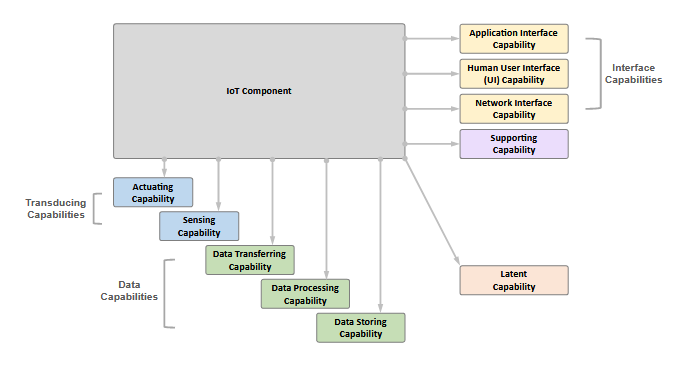
\includegraphics[width=\linewidth]{pic/IIRA-model-component-pattern.png}
	\caption{Component Capability Pattern.}
	\label{fig:Model-Component-Pattern}
\end{figure}
\subparagraph{Three-Tier Architecture Pattern}
The system comprises the Edge, Platform, and Enterprise Tiers, as well as connecting networks. The Edge Tier contains sensors and gateways that collect data. These are connected by the Proximity Network. Data preprocessing may already be happening there.
\\The Platform Tier is responsible for most data processing and storage via databases. It is connected to the Edge Tier via the Access Network.
\\The Enterprise Tier provides domain-specific applications and interfaces for end users. These are built upon the processed data from the platform tier. It also issues controls to lower tiers. This tier is connected to the Access Network via the Service Network.
The three tiers can also be further divided into different domains. That makes sense for bigger systems. But for a symple system as the one described in this work it is not necessary and therefore these domains will be explained here.
\begin{figure}[H]
	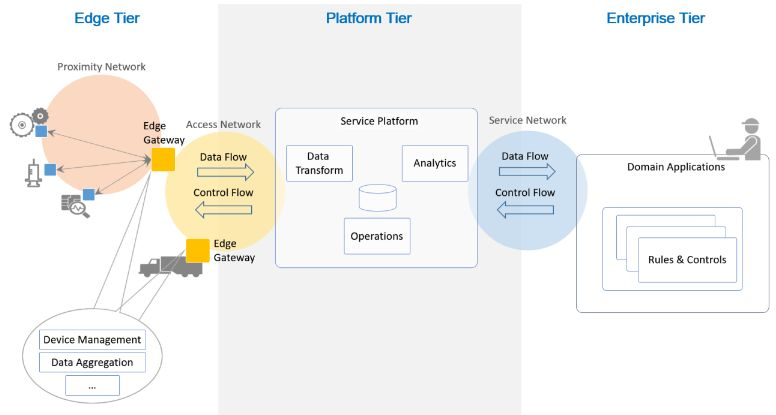
\includegraphics[width=\linewidth]{pic/three-tier-architecture.jpg}
	\caption{Three Tier Architecture}
	\label{fig:Three-Tier-Architecture}
\end{figure}
\subsection{Performance measurement in production environments}
\paragraph{Key Performance Indicators}
The team around \cite{kangHierarchicalStructureKey2016} from the National Institute of Standards and Technologie in the U.S. has worked out the different kinds of KPI's that are being used in operation management and production and how the various metrics and KPI's are related to each other.
\\First there are the supporting elements which in this thesis will be called metrics because they describe the measured data that is needed to calculate the basic KPI's. The supporting elements are devided into the categories time and quantity.
\\Then there are maintenance elements which give insight into upkeep of the machines. Of which the following were able to be calculated with the given metrics.
\\
\subsection{IoT-Plattforms}

\subsection{Databases}
\subsection{Dashboarding}
\addtocontents{toc}{\vspace{0.8cm}}



\clearpage
\chapter{\textbf{Kapitel 3}}\label{kap3}
\addtocontents{toc}{\vspace{0.8cm}}

\begin{table}[htb]
\caption{Messergebnisse}
\label{tab:messung}
\centering
\begin{tabu}{l|[2pt]C|C|C}
Stellung & \frac{T_U}{^\circ C}  & \frac{T_c}{^\circ C} & \frac{\Delta T}{^\circ C}  \\
\tabucline[2pt]{-}
senkrecht (0°) & 27,3 & 69,8 & 42,5\\
\tabucline[0.5pt]{-}
waagerecht (90°) & 26,6 & 70,6 & 44,0\\
\end{tabu}
\end{table}

\begin{table}[h]
\centering
\caption{Smartphone Sensordaten}
\begin{tabu}{|p{9cm}|l|l|}
\hline
Sensorinformation&Format&frequency [$s^{-1}$]\\
\hline
App identifier for vendor & int64 & once per transfer\\
WIFI and network carrier IP addresses& int128 & once per transfer\\
battery level& int8 & 0.1\\
Position information: latitude, longitude, altitude, speed, course, vertical position accuracy, horizontal position accuracy, floor level information& float32[8] & 1\\
Heading information: heading.x, heading.y, heading.z, true heading, magnetic heading, heading accuracy& float16[6] & 1 \\
Accelerometer information: acceleration.x, acceleration.y, acceleration.z& float16[3] & 2 \\
Gyroscope information: rotationRate.x, rotationRate.y, rotationRate.z& float16[3] & 2 \\
altimeter information: relative altitude, pressure & float16[2] & 1 \\ 
timestamp & uint32 & once per transfer \\
Temperature [°C] & float16 & 1\\
\hline
\end{tabu}
\label{tab:smartphonesensor}
\end{table}

Wie in Tabelle \ref{tab:smartphonesensor} zu sehen ist, ist es besser, Trennlinien nur dort einzusetzen, wo logische Grenzen liegen.
\clearpage
\chapter{\textbf{Zusammenfassung und Ausblick}}\label{zusammenfassung}
\addtocontents{toc}{\vspace{0.8cm}}


% Nachspann
\nocite{Segmentation} % Quelle wird nicht im Text erwähnt -> Quellenverzeichnis
\nocite{ImageAttack}
% Weitere quellen müssen in 'bib/quellen.bib' eingetragen werden
% !!! -> BibTex ausführen! Sonst tauchen die Quellen nicht im Verzeichnis auf.

% Quellenverzeichnis
\clearpage
%\bibliographystyle{alpha}
\bibliographystyle{apalike}
\bibliography{./bib/quellen}
\addcontentsline{toc}{chapter}{Quellenverzeichnis}
%\addtocontents{toc}{\vspace{0.8cm}}

% Abkürzungsverzeichnis
\clearpage
\markright{Abkürzungsverzeichnis}
\clearpage
\chapter*{Abkürzungsverzeichnis}\label{abkuerzungsverzeichnis}
\addcontentsline{toc}{chapter}{Abkürzungsverzeichnis}
\begin{acronym}[YTM]
\setlength{\itemsep}{-\parsep}

\acro{IoT}[$IoT$]{\hspace{1cm}Internet of Things}
\acro{IIoT}[$IIoT$]{\hspace{1cm}Industrial Internet of Things}
\acro{KPI}[$KPI$]{\hspace{1cm}Key Performance Indicator}
\acro{PLC}[$PLC$]{\hspace{1cm}Programmable Logic Controller}
\acro{OPC UA}[$OPC UA$]{\hspace{1cm}Open Process Control Unified Architecture}
\acro{DBMS}[$DBMS$]{\hspace{1cm}Database Management System}
\acro{TS-DBMS}[$TS-DBMS$]{\hspace{1cm}Timeseries Database Management System}
\acro{}[$x$]{\hspace{1cm}x}


\end{acronym}

%\addtocontents{toc}{\vspace{0.8cm}}

% Abbildungsverzeichnis
\clearpage
\addcontentsline{toc}{chapter}{Abbildungsverzeichnis}
\listoffigures
%\addtocontents{toc}{\vspace{0.8cm}}

% Tabellenverzeichnis
\clearpage
\addcontentsline{toc}{chapter}{Tabellenverzeichnis}
\listoftables
\addtocontents{toc}{\vspace{0.8cm}}

% Anhaenge
\addcontentsline{toc}{chapter}{Anhang}
\appendix
%\input{./app/Dateiname}
\chapter{Quellcode}
\begin{enumerate}
      \item Source 1
      \item Source 2
\end{enumerate}

% Anhänge im Ordner 'app' ablegen

%\includepdf[pages=1-4]{./app/Datenblatt1.pdf} % Datei mit 4 Seiten
%\includepdf[pages=1]{./app/Datenblatt2.pdf} % Datei mit einer Seite

\chapter{Rohdatenvisualisierungen}
\begin{enumerate}
      \item Graustufen
      \item Verteilungen
\end{enumerate}
\end{document}
